\documentclass[a4paper,12pt]{article}

\usepackage{rotating}
\usepackage[top=1in, bottom=1in, left=1in, right=1in]{geometry}
\usepackage{graphicx}
\usepackage[numbers,square,sort&compress]{natbib}
\usepackage{setspace}
\usepackage[cdot,mediumqspace,]{SIunits}
\usepackage{caption}
\usepackage{subcaption}
\usepackage{mathtools}
\usepackage{authblk}


\begin{document}
\onehalfspacing
\title{The Statistical Behaviour of Photons}
\author{Natalie Price-Jones, with partners Morten Stostad and Lake Marsten}
\date{30 September, 2013}
\affil{\small{natalie.pricejones@mail.utoronto.ca}}
\maketitle

%%%%%%%%%%%%%%
\begin{abstract}
\label{abstract}

The photoelectric effect was made use of through a photomultiplier tube (PMT) to investigate the nature of photon statistics. In this experiment, two statistical models (Poisson and Gaussian) were compared to data taken from a PMT device by its attached counter. In addition, general methods of error reduction and their implementation in observation were explored. As expected, an increased number of samples per observational trial reduced the standard deviation in the measurement of the mean number of photons emitted per time sample. It was also found that the mean value and variance of the number of photon counts have a linear relationship, a hallmark of Poisson statistics. As the length of the time samples was increased, the discrete Poisson distribution for the probability of counts began to merge with the smooth Gaussian distribution.

\end{abstract}

%%%%%%%%%%%%%%
\section{Introduction}
\label{sec:introduction}

This experiment was an exploration of the statistical behavior of photons. The setup was relatively simple $-$ a PMT attached to a device the registers a count when struck by a pulse. The PMT relied on the photoelectric effect, bouncing a single photon from the LED onto multiple dynodes. This process resulted in the photoelectric emission of many electrons due to a single photon. When these electrons reached the detector, they registered as a pulse, and a photon was recorded by the counter.

Using this photon counting device and some Python programs, the data was collected and normalized into count probabilities; the likelihood that a given count number would appear for a sample of set length. These probabilities were compared to Poisson and Gaussian statistical probability distributions to find one that would accurately model the photon behavior. This modeling was then tested at extremes and over multiple trials. The fit was checked both by direct comparison to the data and by less straightforward methods. The latter were mostly reliant on quantifying the relationship between the mean and standard deviation of each data set. These checks combined to fit one statistical model quite effectively, especially when conditions were placed upon the mean.

\section{Observations and Data}
\label{sec:observations}

The primary acquisition device used in this experiment was the PMT and attached USB-4301 counting device. The setup had only rudimentary controls: an overall power switch, a switch to turn the lamp on and off, and an unlabeled brightness dial.  An associated python script called PMT.py was provided to gather data from the photon counter as an array. This program contained a function called photoncount that took two arguments: the number of time samples (nsamp), and the length of each sample (tsamp). After recording counts for a length of time equal to nsamp multiplied by tsamp, the function returned an array of numbers representing the number of photons counted during the time specified for each sample.

Observations were undertaken over the course of two weeks when the entire lab team could be present. Only one or two group members recorded data (see Table~\ref{tab:datatable}), but each individual analyzed the resulting output in its graphical form. Together, it was decided whether the data sets collected were in keeping with predictions or if there were inexplicable discrepancies.

\begin{center}
  \begin{table}[h]
  \centering
  \begin{tabular}{p{1.5in}||p{2.5in}||l}
    Name of Recorder & Section Recorded For & Date Recorded\\
    \hline
    Lake Marsten & Section 4 (tsamp = 0.001; nsamp = 100) & September 23 2013\\
    \hline
    Morten Stostad and Natalie Price-Jones & Section 5 (tsamp = 0.01; nsamp = 100; 6 repetitions) & September 23 2013\\
    \hline
    Morten Stostad and Natalie Price-Jones & Section 6 (tsamp = 0.01; nsamp = 100, 500, 1000; 2 repetitions) & September 23 2013 \\
    \hline
    Natalie Price-Jones & Section 7 (tsamp = 0.001, 0.005, 0.01, 0.05, 0.1; nsamp = 100; 2 repetitions) & September 18 2013\\
    \hline
    Natalie Price-Jones & Section 8 (tsamp = 0.03, 0.3; nsamp = 1000; 6 and 4 repetitions for each tsamp respectively) & September 23 2013\\
    \hline
    Natalie Price-Jones & Section 9 (tsamp = 0.01s; nsamp = 2, 4, 8, ..., 512, 1024; 15 repetitions of each nsamp)& September 27 2013\\
    \end{tabular}
    \caption{Personnel who recorded data for each section of the lab handout}
    \label{tab:datatable}
  \end{table}
\end{center}
Since some data sets were taken with a gap of days between each session, efforts were made to ensure that external conditions were similar. However, since the brightness dial on the PMT was unmarked, it was difficult to record completely consistent data. Ideally, the situation would have been such that only the parameters sent to PMT.py would have changed between each step.

Often, the PMT itself would experience problems. Even when the light was off, some count activity was expected, but for long stretches the PMT would simply output zero arrays. When running a loop that gathered many data sets at once, the start of this behavior was not always obvious and had the potential to ruin the set. Another error with the machine or its partner software caused it to report counts in excess of several thousand, regardless of the length of the sample time. This was even more challenging to identify, as only a few counts were misreported, though the fix in this case was to simply remove outlying points.

As mentioned above, the counter reported photons even when the light was off in the PMT. There are a few reasons for this: first that the PMT was not perfectly insulated, and so some stray photons might have made it in from the outside. In addition, the PMT was at room temperature. For everyday materials, 273K is not hot enough to give an electron the energetic kick it needs to escape its bonds (E = $\frac{3}{2}$kT where k is the Boltzmann constant and T is temperature). However, by virtue of the sheer number of electrons and thermodynamic probabilities, some may have escaped and caused a false report of a photon. 

\section {Data Reduction and Methods}
\label{sec:methods}

Data was analyzed using the Python language, largely with original functions written for the task. Plotting the data at every step was done with the pyplot module, part of matplotlib.

The first part of the analysis done for this experiment was mostly concerned with plotting data and developing intuition for expected outcomes. Plotting raw count data against time was uninformative (see Figure~\ref{fig:section4}), so a function was written to convert the array of counts into a histogram. It was simply a matter of finding how many times a given number of counts was recorded and plotting that information against the count value. This proved to be much more relevant than the original plot of the number of counts over time.

\begin{figure}[h]
\centering
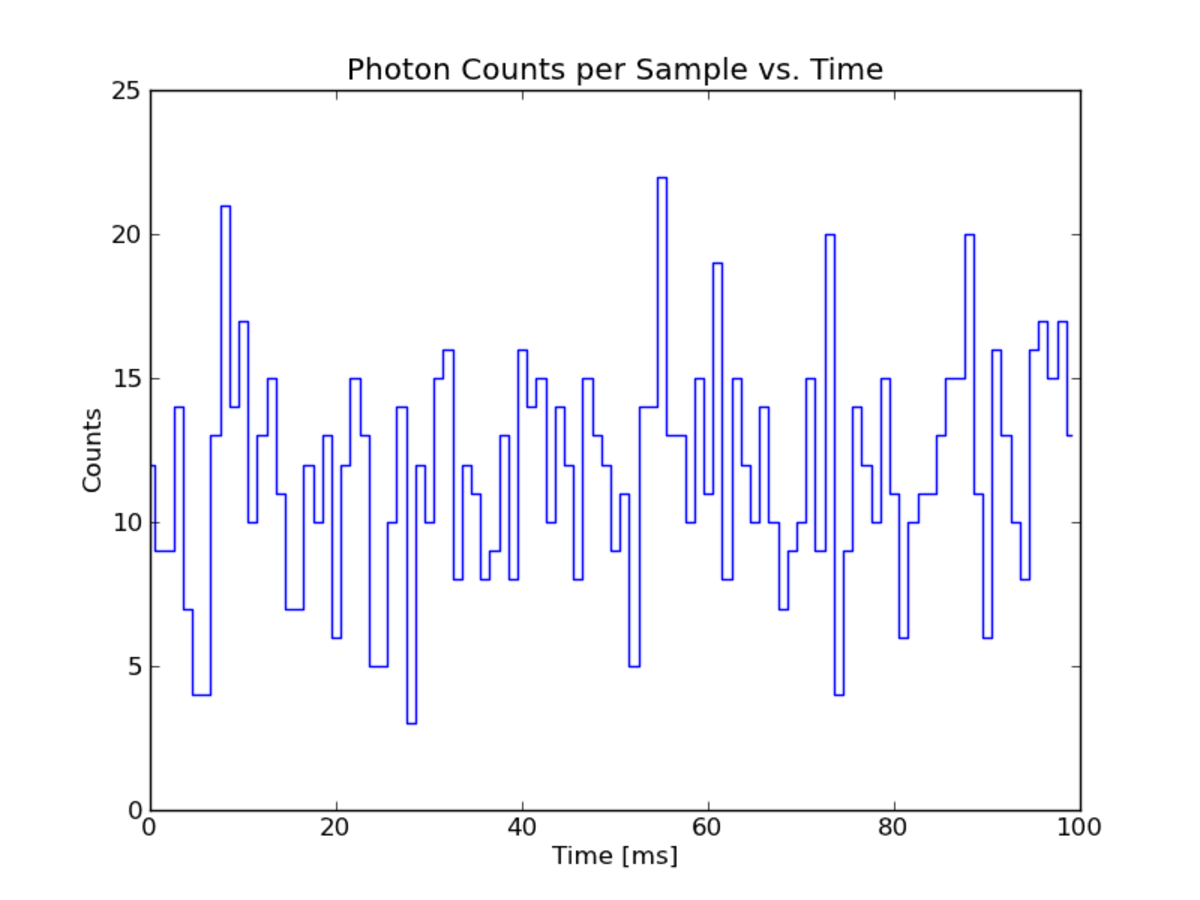
\includegraphics[width=\linewidth]{section4image.pdf}
\caption{An example of raw data from the Photon Multiplier Tube, where the sample time was 0.001 seconds and 100 samples were taken.}
\label{fig:section4}
\end{figure}

After using the histogram function to plot count frequency for varying parameters, the next step was to make some statistical predictions. This required writing two new functions: one for a Poission distribution, and another for a Gaussian distribution. In addition, it was necessary to calculate the mean and standard deviation of the data sets. The actual formulae are outlined below in Section~\ref{sec:calculations}, but the functions needed were not so complex as to be challenging to model. Due to the limitations of the written factorial function needed for the Poisson distribution, it was necessary to use the scipy.stats Poisson function on data sets with a high number of counts per sample.

Both of the distributions listed above provide output as probability, so a final modification to the raw data was necessary. Rather than plot just the frequency of counts, as in Figure~\ref{fig:histograms}, each such frequency was normalized by dividing it by the total number of counts recorded. This provided the probability of finding a certain number of counts. 

The final matter of concern with regard to the methods were possible sources of error (as outlined in Section~\ref{sec:observations}). Of particular concern were systematic dark counts, the photon counts recorded when the LED in the PMT was turned off. After some measurements taken when the light in the room containing the PMT was both on an off, it was found that the counter was averaging 81 counts per second. Later measurements of dark counts clocked in at 50 $\pm{ 20}$ counts per second. Such fluctuation seemed to be typical, and was not quatitatively accounted for in the following sections.

\section{Calculations and Modeling}
\label{sec:calculations}

The instructions for modeling the behavior of the photon counts were provided in the lab handout, but required some tweaking to achieve the desired results. This was  particularly true of the python implementation. One of the most significant challenges was comprehending the behavior of the probability functions and understanding each of the variables.

The first step towards plotting either of the probability distributions was calculating the mean ($\mu$) and standard deviation ($\sigma$) - Equations~\ref{eqn:mean}, and~\ref{eqn:standard deviation} respectively. 


\begin{equation}
\label{eqn:mean}
\mu = \frac{\sum_{i=1}^{N}{x_i}}{N}
\end{equation}

Here, the mean is simply the sum of the data points ($x_i$) divided by the number of data points (N).

\begin{equation}
\label{eqn:standard deviation}
\sigma = \sqrt{\frac{\sum_{i=1}^{N}(x_i-\mu)^2}{N-1}}
\end{equation}

The standard deviation is the square root of the sum of the squared deviation of each $x_i$ from the mean divided by the number of data points minus one. The squared deviation is necessary to avoid negative values, the N-1 to account for the fact that while all of the data points are independent of each other, none is independent from itself.
\\
\\
With this information, and the histogram modified to display probabilities, it was possible to overplot the Poisson and Gaussian distributions (Equations~\ref{eqn:poisson} and~\ref{eqn:gaussian} respectively).

\begin{equation}
\label{eqn:poisson}
P(x;\mu) = \frac{\mu^x}{x!}exp(-\mu)
\end{equation}
It is interesting to note that the Poisson distribution (unlike the Gaussian distribution), does not take standard deviation into account. Instead, it bases the standard deviation on the mean ($\sigma$=$\sqrt{\mu}$). This relationship was later demonstrated in the photon data, as in Figure~\ref{fig:section7}. The other relevant feature of the Poisson distribution is its discrete nature. Since it depends on the factorial of x, it is only meaningful for integer values. This makes sense for a photon count distribution, where the number of counts per time sample is necessarily discrete in order to be physically sensible.

\begin{equation}
\label{eqn:gaussian}
P(x;\mu,\sigma) = \frac{1}{\mu\sqrt{2\pi}}exp[-\frac{1}{2}(\frac{x-\mu}{\sigma})^2]
\end{equation}

The Gaussian distribution is more widely applicable than the Poisson distribution in that it is continuous. However the question remained as to whether it was a good fit for the photon data collected over the course of this experiment.

Calculations using the above equations were done entirely through python.

\section{Discussion}

The first step of the investigation was to test the PMT and get a sense for reasonable output. To this end, data was recorded at the same tsamp and nsamp values with six repetitions (see Figure~\ref{fig:section5} for three of these repetitions). The shape of histogram varies considerably, despite the data having been recorded with the same input parameters. This speaks the randomness of the process, especially at a low number of samples. In the adjacent set of plots, Figure~\ref{fig:section6}, the number of samples was increased with each iteration. Here, the shape of the histogram becomes more regular, peaking towards the mean with less fluctuation.

\begin{figure}[h]
\begin{tabular}{c|c}
\centering
\begin{subfigure}{0.5\textwidth}
  \centering
  \hspace{-0.3in}
  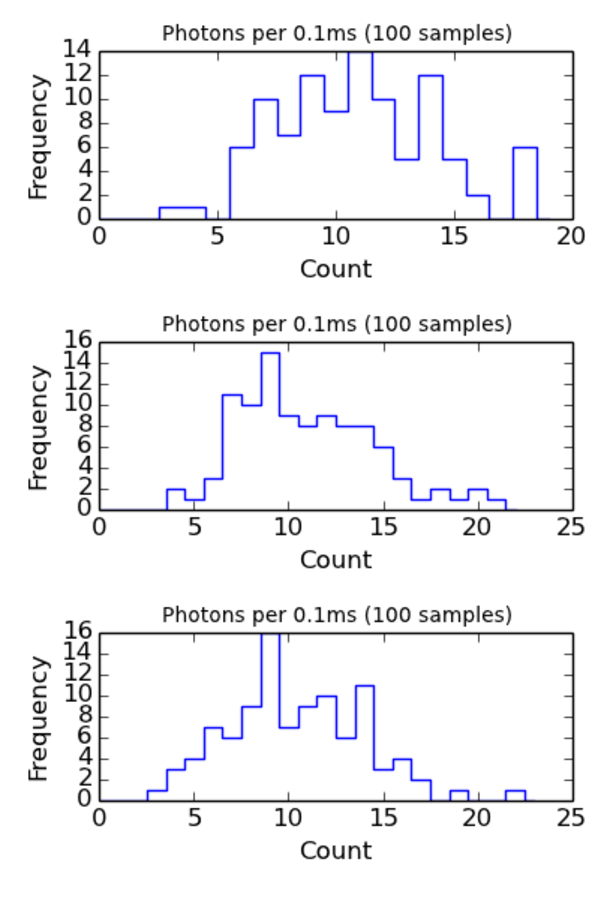
\includegraphics[width=\linewidth]{section5_crop.pdf}
  \captionsetup{justification=centering}
  \caption{An example of the variety of \\histogram shapes at a relatively low number \\of samples.}
  \label{fig:section5}
\end{subfigure}
\end{tabular}
\begin{subfigure}{0.5\textwidth}
  \centering
  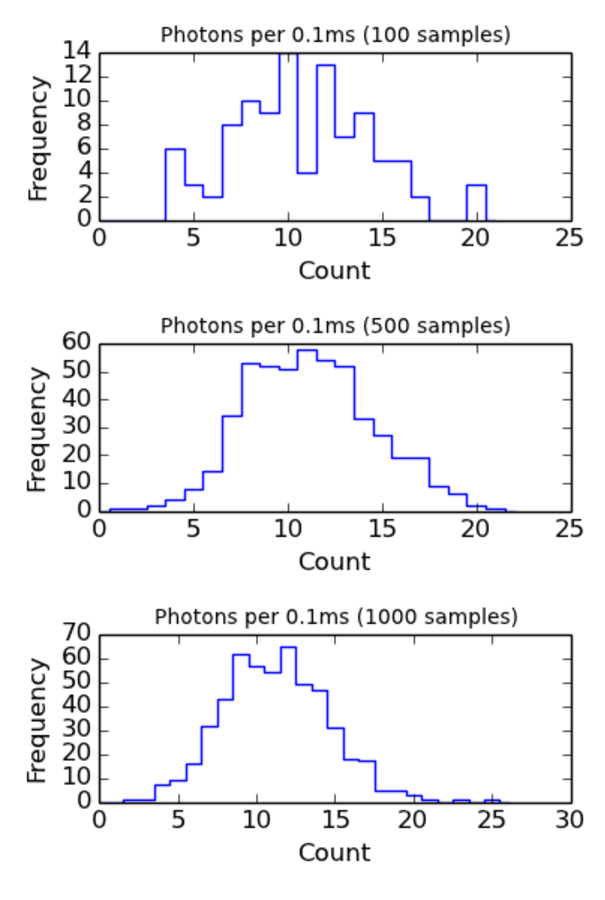
\includegraphics[width=1\linewidth]{section6_crop.pdf}
  \captionsetup{justification=centering}
  \caption{A demonstration of the evolution of \\histogram shape as the number of samples \\increases.}
  \label{fig:section6}
\end{subfigure}%
\caption{Histogram trends for the same sample time with varying numbers of samples.}
\label{fig:histograms}
\end{figure}

Once the standard count behavior was clear, the next task was to develop a fit to the data. To do this, the mean and standard deviation (Equation~\ref{eqn:standard deviation}) were calculated for six data sets with increasing tsamp values. It was assumed that since the lower limit on tsamp was 0.0001s, and data was recorded starting at 0.001s and increasing by amounts 0.001s or larger, the quantization of sample time would not significantly effect the data.

The mean increased with the length of the sample, as would be expected (a longer time means more photon counts per sample), but so did the standard deviation. This is not as surprising as it had initially seemed; a longer sample times allows for more fluctuation in count values (compare Figure~\ref{fig:section8ms} and~\ref{fig:section8s}, for example). The variance, which is simply the square of the standard deviation, was plotted against the mean count value, on both a linear and log scale (Figure~\ref{fig:section7}). The overplotted x=y fit makes it clear that the two variables are linearly related. A linear relation between variance and mean value implies that standard deviation is proportional to the square root of the mean, a requirement to fit Poisson statistics.

\begin{figure}[h]
\centering
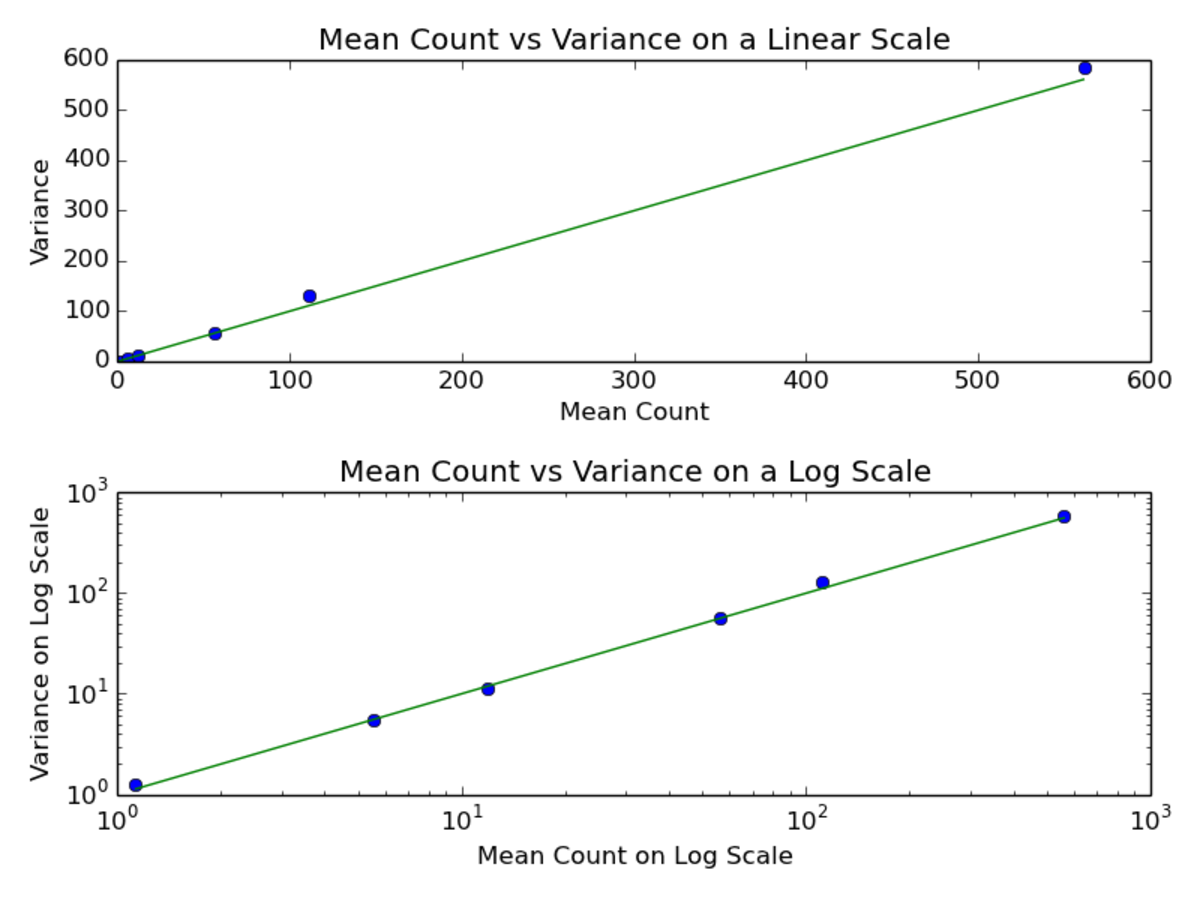
\includegraphics[width=\linewidth]{section7.pdf}
\caption{Mean number of counts plotted against variance for increasingly long time samples at 100 samples each. The blue points are the data, the green line a linear fit.}
\label{fig:section7}
\end{figure}

As the mean increases, however, it is clear on the linear plot that the scatter away from the linear fit is also increasing (albeit on a small scale). This implies that the relationship between standard deviation and mean dictated by Poisson statistics might not hold as well for larger means. However, this possible departure from Poisson statistics is not completely determined just by analysing Figure~\ref{fig:section7}. On the linear plot, the points representing small time scales are clustered near the origin, and it is difficult to discern how far they might scatter from the fit line. The scatter at higher means is hardly present on the log scale plot. Clearly a more exhaustive check of photon behavior is needed to posit that Poisson statistics do not hold for large means.

The claim was further investigated by comparing two sets of count data taken over 0.3s and 0.003s times at 1000 samples each. Each set was plotted as a histogram, with Poisson (Equation~\ref{eqn:poisson}) and Gaussian (Equation~\ref{eqn:gaussian}) statistical predictions plotted over top based on the mean and standard deviation of the set (see Figure~\ref{fig:section8}). 

\begin{figure}[h]
\centering
\begin{subfigure}{\textwidth}
  \centering
  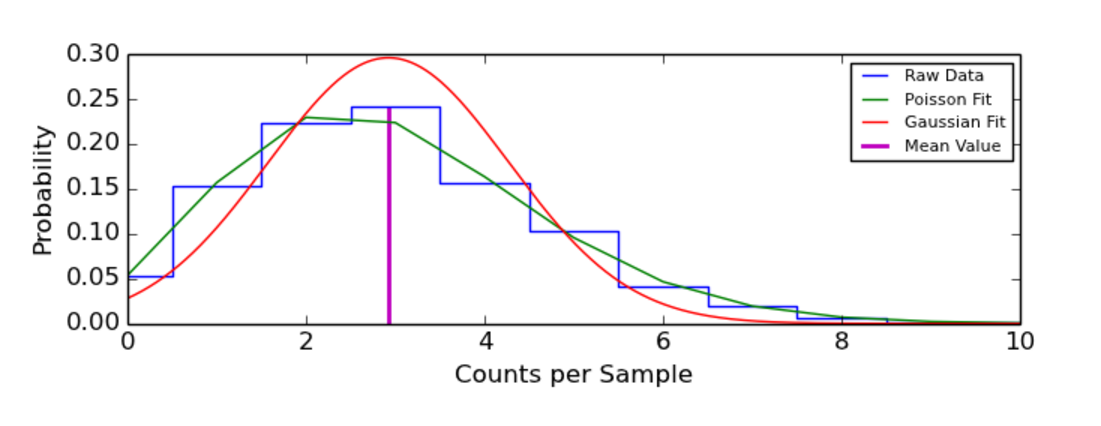
\includegraphics[width=\linewidth]{3ms_section8_2_crop1.pdf}
  \vspace{-0.25in}
  \caption{Sample time 3ms, with a total of 1000 samples.}
  \label{fig:section8ms}
\end{subfigure}%
\qquad
\begin{subfigure}{\textwidth}
  \centering
  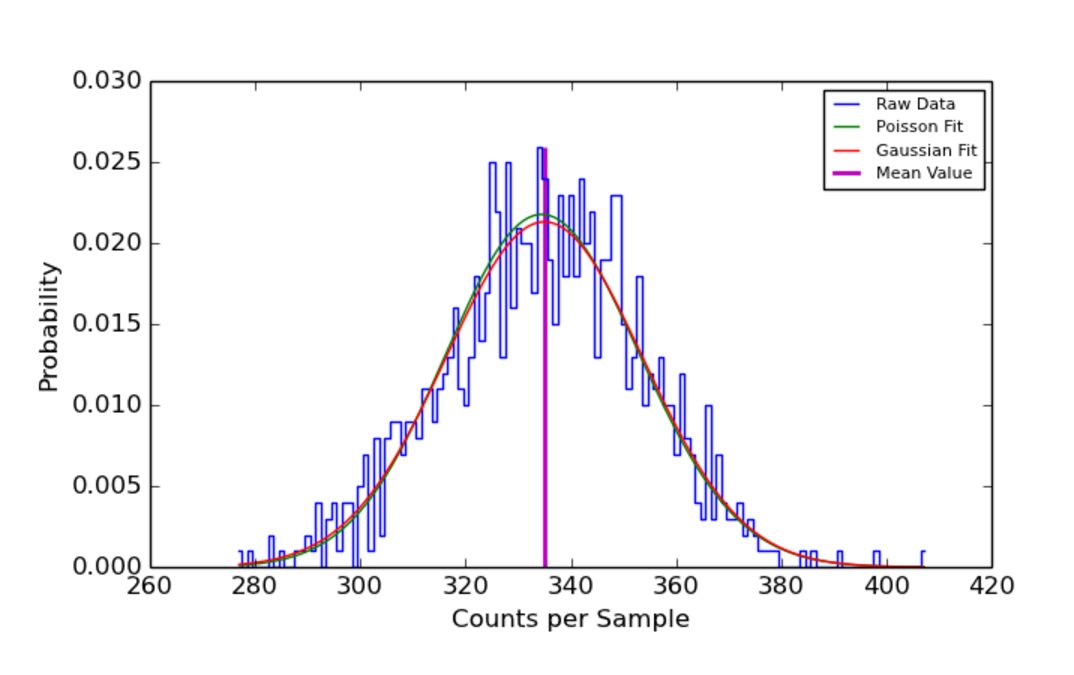
\includegraphics[width=\linewidth]{s_section8_2_crop1.pdf} 
  \vspace{-0.25in}
  \caption{Sample time 0.3s, with a total of 1000 samples.}
  \label{fig:section8s}
\end{subfigure}%
\caption{Histograms of the probability of count number with over plotted fits from Poisson and Gaussian statistics.}
\label{fig:section8}
\end{figure}

A few qualitative features are immediately obvious. As was previously established, a higher mean value means higher count values and standard deviation. In keeping with this, Figure~\ref{fig:section8s} has a wider and more symmetric distribution than its shorter timescale counterpart. Of course, Figure~\ref{fig:section8ms} lacks symmetry partly because its mean value is so close to zero, and obviously a count of less than zero photons points to a device malfunction, not a physical phenomenon.



More striking is the difference between the fits for each plot. In the first, it is clear that the Poisson prediction much better describes the data, matching far closer to the measured data than the high-peaked Gaussian curve. However, in the second plot,  the two predictions of probability are nearly the same curve, and both a reasonable description of the data. In the case of the longer sample time, the count probability fluctuates more extremely, but overall follows a standard normal distribution. It appears that a Gaussian probability distribution is a good approximation of both the data and a Poisson distribution for high enough means.

However, photon statistics at low mean values are clearly well described by the Poisson distribution, where the mean value determines the fit. The next matter of concern was how to refine this mean value to greater precision.

\begin{figure}[h]
\centering
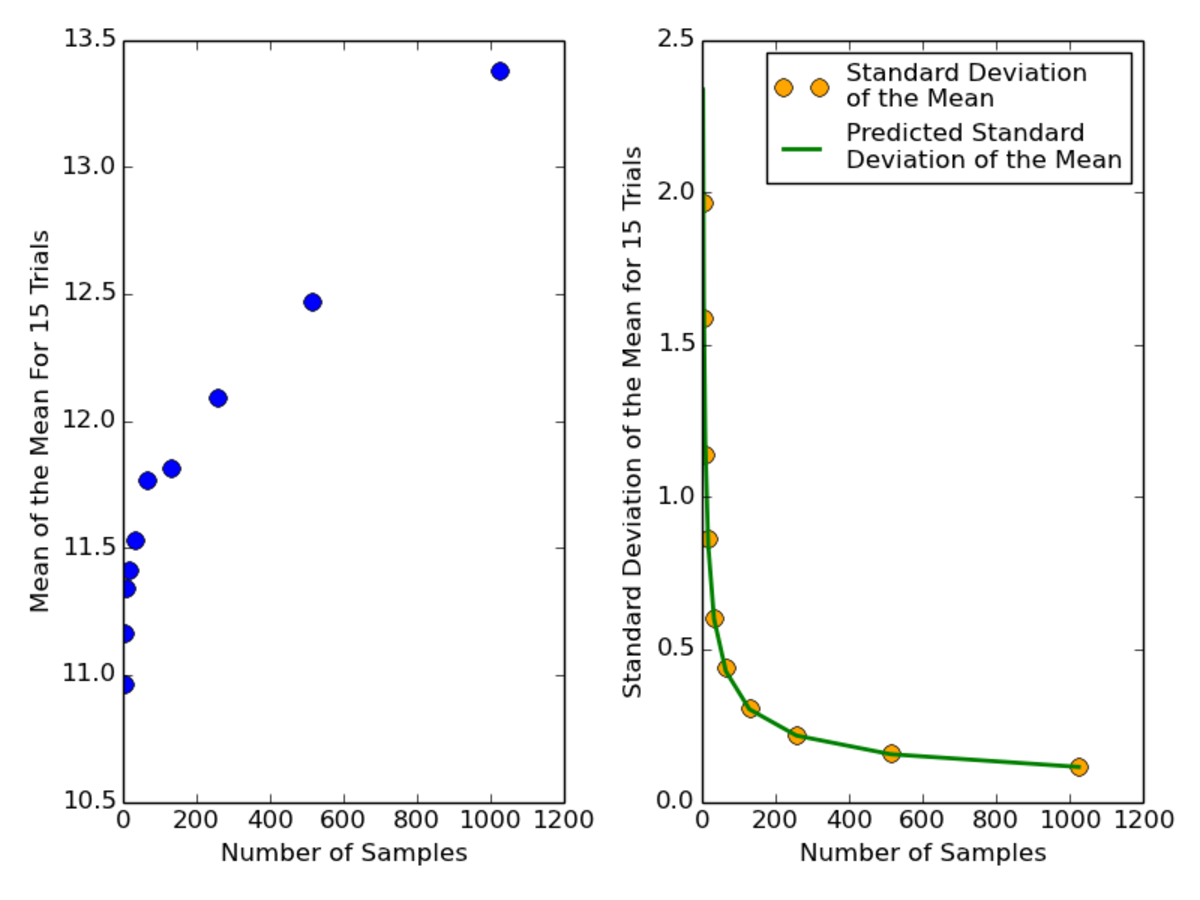
\includegraphics[width=\linewidth]{section9_fix.pdf}
\caption{Mean of means and standard deviation of means as the number of samples increases, with 15 trials at each number of samples. Each sample was 0.01s long. The predicted fit is based on Poisson statistics.}
\label{fig:section9}
\end{figure}

Obviously, there are systematic errors associated with the PMT, but the aim was to minimize the statistical error of the measurements. To this end, data was taken with a 0.01s sample time and a number of samples that increased by a power of two with each repetition. For each nsamp value, fifteen data sets were recorded. A mean value and standard deviation were calculated for each set, and from these fifteen values, a mean of the means (MOM) and a standard deviation of the means (SDOM) was calculated. In Equation~\ref{eqn:sdom}, $\sigma_\mu$ is the standard deviation in the mean and N is the number of samples. 

\begin{equation}
\label{eqn:sdom}
\sigma_\mu=\frac{\sigma}{\sqrt{N}}
\end{equation}


It was expected that the mean of the means would approach a relatively constant value and the standard deviation of the means would decrease as nsamp increased. Fluctuations were expected for low nsamp values, but since the photon measurement has been shown to be a statistical, not random, process, more measurements should increase the precision of the calculated data. However, this prediction does not entirely match the recorded data. Figure~\ref{fig:section9} shows the results of plotting the MOM and SDOM values against the number of samples used in the calculation. Contrary to expectations, the MOM increases with nsamp, though not in any predictable way. Since the data taken to form this plot was taken in succession with no interference with PMT controls, it is likely that this effect is due to the systematic errors of the setup (or dark counts, as they have been referred to previously).

The SDOM values do match expected behavior, fitting remarkably well to predicted values. These predictions were based on the accuracy of Poisson statistics in fitting earlier data (Figure~\ref{fig:section8}). In Poisson statistics, the standard deviation is simply the root of the mean. For each of the fifteen sets for a given nsamp value, the square root of the mean was calculated according to $\sigma = \sqrt{\mu}$. From these predicted values, the SDOM was calculated with Equation~\ref{eqn:sdom} as with the raw data.  The SDOM values decrease sharply as the number of samples increases. This is quite logical, as the SDOM is inversely proportional to the number of samples. However, the increase in precision begins to slow down even as nsamp continues to increase, because the proportionality is limited to the square root of nsamp. Increasin nsamp by a factor of four will only improve precision by a factor of two. It is clear that after a certain nsamp, increasing the number of samples no longer results in a significant reduction in standard deviation.

Once this threshold is reached, might it be possible to eliminate the systematic error plaguing the MOM plot in Figure~\ref{fig:section9}? The goal would be to construct a light source that exhibits no variation, always providing a uniform count rate. Common sense dictates this is impossible - and indeed it is. There is no way to remove quantum fluctuations from the equation, even if one were to better insulate and cool the source to reduce the number of wayward electrons.

At the moment, however, the primary avenue of further investigation would still be an attempt to locate a more regular and less intrinsically faulty PMT device, in hopes of getting more consistent MOM data. A more thorough exploration of the inherent noise in the source would also help in the analysis of the data. For the moment, information recorded so far does point strongly to photon counting with a PMT being well described with Poisson statistics, or Gaussian statistics at high means.




\bibliographystyle{plainnat}
\bibliography{cite}

\end{document}